\chapter{SYSTEM ARCHITECTURE} \label{chap_sys_architecture}
System architecture is explained and analyzed under three sub sections.
\begin{enumerate}
    \item Main overview of the system is explained in the Section \ref{sec_overview_sys_architecture}.
    \item Hardware design and architecture is explained in the Section \ref{sec_hardware_design}.
    \item Firmware design and architecture is explained in the Section \ref{sec_firmware_design}
    \item SİLİNECEK \cite{One, Two, Three}.
    
\end{enumerate}

\section{Overview of the System Architecture} \label{sec_overview_sys_architecture}

The system consist of paired RC car and Android phone. Android phone, which runs the remote control interface, connects the target RC car unit via Bluetooth communication and send / receive control packets over this channel. At server (database) side, each Android\texttrademark\;phone connects to the Firebase database in order to establish an online session for game. Figure \ref{fig:overview_architecture} shows the diagram of the main system architecture.

\begin{figure}[!htbp]
    \centering
    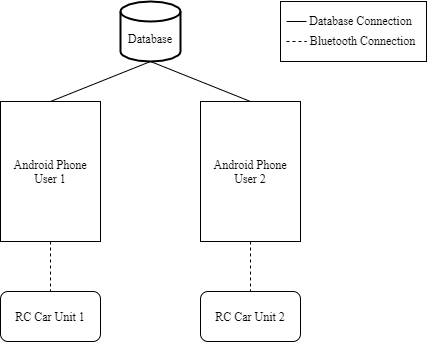
\includegraphics[width=0.8\textwidth]{Imgs/overview_of_sys.drawio.png}
    \caption{\label{fig:overview_architecture}Diagram of the Main System Architecture}
\end{figure}

\section{Hardware Design} \label{sec_hardware_design}

\subsection{Hardware Architecture} \label{sec_hardware_architecture}

Main hardware architecture and power / harness diagram is shown in Figure \ref{fig:hardware_architecture}. 

\begin{figure}[!htbp]
    \centering
    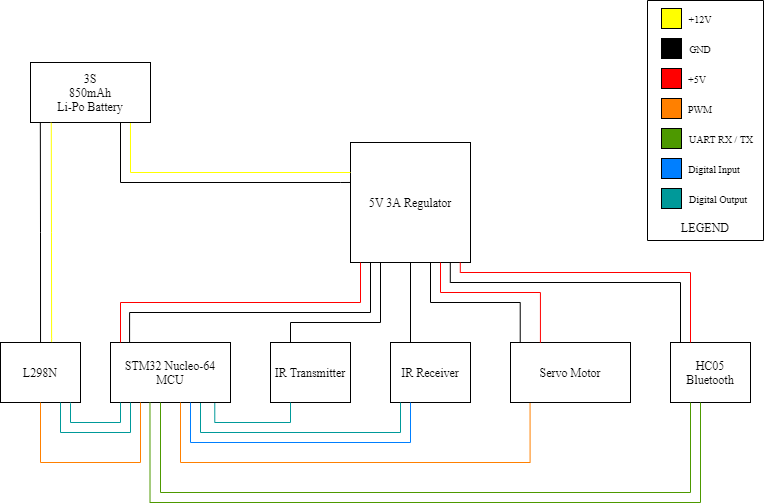
\includegraphics[width=1\textwidth]{Imgs/ana_devre_v3.png}
    \caption{\label{fig:hardware_architecture}Power / Harness Diagram of the Hardware}
\end{figure}

Explain system here....

% Hardware Components Part Start
\noindent \textbf{STM32 MCU} \\
The system uses STM32 Nucleo-64 development board as a MCU of the RC car unit. STM32 Nucleo-64 development board is based on processor Arm\textregistered\;Cortex\textregistered\;M4, has 32.768 kHz crystal oscillator,  has 11 timers: up to six 16-bit, two 32-bit timers up to 100 MHz, has 512 Kbytes of flash memory and 128 Kbytes of SRAM \cite{One}. This MCU provides necessary peripherals and clock speed for the RC car unit. This board has built-in ST link programming interface and driver which provides fast development without additional ST link device. The implementation of the hardware and firmware is not restricted with this development board, similar approach can be applied with any MCU that is based on Arm\textregistered\;Cortex\textregistered\;M4 family and that has sufficient number of timers, GPIOs and other essential peripherals. This development board is shown in Figure \ref{fig:nucleo64_board}.\\

\begin{figure}[!htbp]
    \centering
    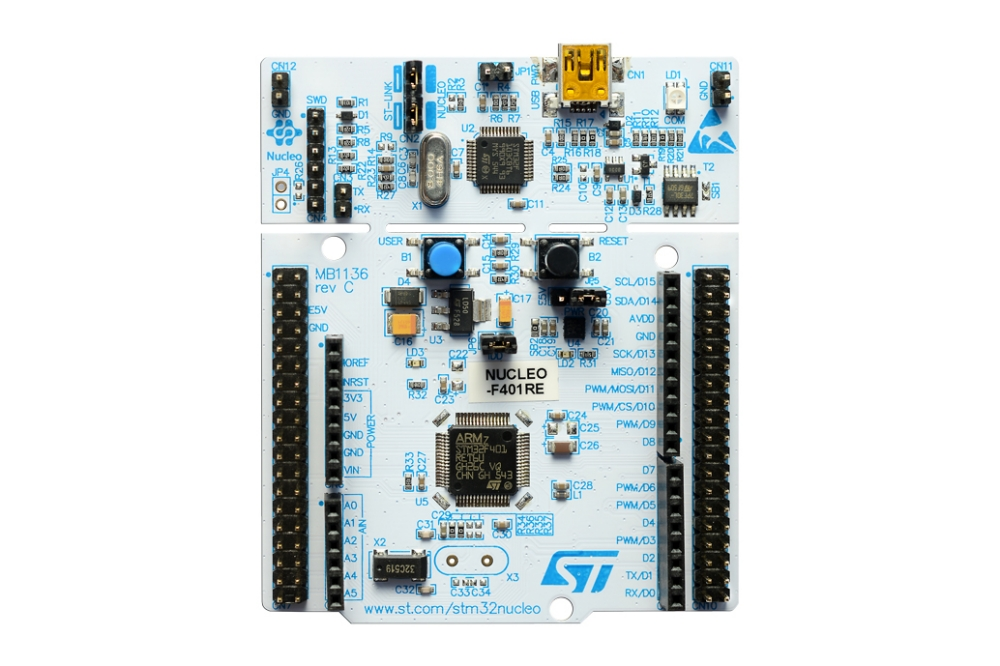
\includegraphics[width=0.8\textwidth]{Imgs/nucleo64.jpg}
    \caption{\label{fig:nucleo64_board}STM32 Nucleo-64 Development Board \cite{One}}
\end{figure}

\noindent \textbf{L298N DC Motor Driver} \\
STMicroelectronics\texttrademark\;L298N dual full bridge DC motor driver is used for driving the DC motor of the RC car unit. It is a high voltage, high current dual full-bridge driver designed to accept standard TTL logic levels and drive inductive loads such as relays, solenoids, DC and stepping motors. Two enable inputs are provided to enable or disable the device independently of the input signals. This enable inputs accepts PWM signals for driving motors with speed control. The L298N motor driver accepts 5-46V supply, provides maximum 2A DC current per channel \cite{Two}. According to these specifications and power ratings, this motor driver meets the requirements of the RC car unit. Motor driver PCB is show in Figure \ref{fig:l298n_pcb} .

\begin{figure}[!htbp]
    \centering
    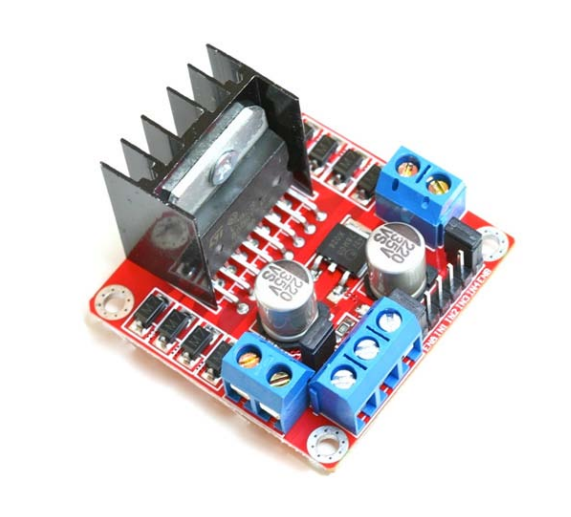
\includegraphics[width=0.5\textwidth]{Imgs/l298n.png}
    \caption{\label{fig:l298n_pcb}L298N Motor Driver PCB}
\end{figure}


\noindent \textbf{Voltage Regulator} \\
LM2596 3-A Step-Down Voltage Regulator is used for powering the system components which accept 5V for supply voltage. MCU, servo motor and HC05 Bluetooth\texttrademark\;module are powered from voltage regulator output. The LM2596 series of regulators are monolithic
integrated circuits that provide all the active functions for a step-down (buck) switching regulator, capable of driving a 3-A load with excellent line and load
regulation \cite{Three}. This voltage regulator supplies enough output current for powering the 5V components in the system.

\noindent \textbf{HC05 Bluetooth Module} \\
The Bluetooth\texttrademark\;wireless technology is designed as a short-range networking solution for personal, portable electronic devices and embedded systems. It overcomes the limitations of line of sight and one to one communication of its possible competitor Infra-Red(IR). It operates in the 2.4 GHz Industrial, Scientific and Medical (ISM) band at a maximum data rate of 720 Kbps \cite{Bluetooth_Overview}. \\

In RC Car Battle system, Bluetooth\texttrademark\;is used for communication between the RC car unit and the remote controller Android\texttrademark\;phone. 

\noindent \textbf{IR Transmitter and Receiver Module} \\
asd
% Hardware Components Part End


\subsection{RC Control Unit}
asd
The Algorithm \ref{labelOfAlgorithm} shows the pseudo code of...
\begin{algorithm}
\caption{Caption of the algorithm}
\label{labelOfAlgorithm}
\begin{algorithmic}
\Require $n \geq 0$ % i.e. input
\Ensure $y = x^n$  % i.e. output
\State $y \gets 1$
\State $X \gets x$
\State $N \gets n$
\While{$N \neq 0$}
\If{$N$ is even}
    \State $X \gets X \times X$
    \State $N \gets \frac{N}{2}$  \Comment{This is a comment}
\ElsIf{$N$ is odd}
    \State $y \gets y \times X$
    \State $N \gets N - 1$
\EndIf
\EndWhile
\end{algorithmic}
\end{algorithm}

\section{Firmware Design} \label{sec_firmware_design}

\subsection{Bidirectional Reliable Bluetooth Communication} \label{sec_bluetooth_comm}

\subsection{Controlling Motors} \label{sec_controlling_motors}

\subsection{IR Receiver and IR Transmitter} \label{sec_ir_rx_tx}

\subsection{Reading Li-Po Battery Voltage} \label{sec_read_lipo_voltage}

\subsection{Main Overview of the System Components} \label{main_system_components}



\begin{comment}
% Below are comments, just for source..
    Ut enim ad minima veniam, quis nostrum exercitationem ullam corporis suscipit laboriosam, nisi ut aliquid ex ea commodi consequatur? Quis autem vel eum iure reprehenderit qui in ea voluptate velit esse quam nihil molestiae consequatur, vel illum qui dolorem eum fugiat quo voluptas nulla pariatur? \ref{tab:widgetss}

    \begin{table}[!htbp]
    \centering
    \caption{\label{tab:widgetss}Comparison of percentages.}
    \begin{tabular}{c|cc|cc}
    \hline
    Mode &  \multicolumn{2}{c}{Var} & \multicolumn{2}{c}{Cum}\\ 
    \hline
    1   &  17.5 & 19.1   & 17.5  & 19.1\\
    2   &  11.8 & 12.7   & 29.3  & 31.9\\
    3   &  6.6  &  5.6   & 35.9  & 37.4\\
    \end{tabular}
    \end{table}
    
    \begin{enumerate}
    \item first,
    \item second.
    \end{enumerate}
    \dots and bullet points \dots
    \begin{itemize}
    \item one bullet,
    \item two bullets.
    \end{itemize}
    
    Let $X_1, X_2, \ldots, X_n$ be a sequence of independent and identically distributed random variables with $\text{E}[X_i] = \mu$ and $\text{Var}[X_i] = \sigma^2 < \infty$, and let
    \[S_n = \frac{X_1 + X_2 + \cdots + X_n}{n}
          = \frac{1}{n}\sum_{i}^{n} X_i\]
    denote their mean. Then as $n$ approaches infinity, the random variables $\sqrt{n}(S_n - \mu)$ converge in distribution to a normal $\mathcal{N}(0, \sigma^2)$.
    
    \begin{quote}
        At vero eos et accusamus et iusto odio dignissimos ducimus qui blanditiis praesentium voluptatum deleniti atque corrupti quos dolores et quas molestias excepturi sint occaecati cupiditate non provident, similique sunt in culpa qui officia deserunt mollitia animi, id est laborum et dolorum fuga.
    \end{quote}
\end{comment}